\documentclass[12pt]{article}

\usepackage[utf8]{inputenc}
\usepackage[a4paper,margin=1in]{geometry}
\usepackage{graphicx}
\usepackage{amsmath}
\usepackage{hyperref}
\hypersetup{
    colorlinks=true,
    linkcolor=blue,
    urlcolor=blue,
    citecolor=black
}
\usepackage{listings}
\usepackage{xcolor}
\usepackage{float}

%----------------------------------------
% Code Style
%----------------------------------------
\definecolor{codegreen}{rgb}{0,0.6,0}
\definecolor{codegray}{rgb}{0.5,0.5,0.5}
\definecolor{codepurple}{rgb}{0.58,0,0.82}
\definecolor{backcolour}{rgb}{0.95,0.95,0.92}

\lstdefinestyle{mystyle}{
    backgroundcolor=\color{backcolour},
    commentstyle=\color{codegreen},
    keywordstyle=\color{magenta},
    numberstyle=\tiny\color{codegray},
    stringstyle=\color{codepurple},
    basicstyle=\ttfamily\footnotesize,
    breaklines=true,
    captionpos=b,
    keepspaces=true,
    numbers=left,
    numbersep=5pt,
    showspaces=false,
    showstringspaces=false,
    showtabs=false,
    tabsize=2
}

\lstset{style=mystyle}

%----------------------------------------
% Title
%----------------------------------------

\title{\textbf{
Analyzing and Mitigating Overfitting in Neural Networks using MNIST}}

\author{
Aaron Roy\\
B.Tech Computer Science Engineering\\
Saintgits College of Engineering
}

\date{\today}

%----------------------------------------

\begin{document}

\maketitle

\tableofcontents

\newpage

%----------------------------------------
\begin{abstract}
This report presents an experiment that intentionally overfits a Multi-Layer Perceptron (MLP) on the MNIST handwritten digit dataset and then demonstrates how regularization techniques improve the model's ability to generalize. The project is divided into two phases. The first phase trains a high-capacity neural network without any regularization, while the second phase applies Data Augmentation and $L_2$ Regularization (Weight Decay) to reduce overfitting and improve validation performance.
\end{abstract}

\newpage

%----------------------------------------

\section{Introduction}

Overfitting is one of the most common problems in machine learning. It occurs when a model memorizes the training dataset instead of learning meaningful patterns. Although such a model performs exceptionally well on training data, it performs poorly on unseen data.

The objective of this project is to intentionally create an overfitted neural network using the MNIST dataset and then demonstrate how standard regularization techniques improve the model's generalization ability.

%----------------------------------------

\section{GitHub Repository}

The complete implementation, source code, training scripts, and model are available in the GitHub repository below.

\bigskip

\textbf{GitHub Repository:}

\url{https://github.com/aaronroy123/task1}



%----------------------------------------

\section{Methodology}

\subsection{Dataset Preparation}

The project uses the MNIST handwritten digit dataset.

The dataset contains grayscale images of size $28\times28$ pixels representing handwritten digits from 0 to 9.

The dataset is divided into:

\begin{itemize}
    \item Training Set: 50,000 images
    \item Validation Set: 10,000 images
    \item Test Set: 10,000 images
\end{itemize}

Two different preprocessing pipelines were used.

\subsubsection{Phase 1}

The images are converted into tensors and normalized using

\[
Mean = 0.1307
\]

\[
Standard\ Deviation = 0.3081
\]

No augmentation is performed.

\subsubsection{Phase 2}

The training images are augmented using

\begin{itemize}
    \item Random Rotation (15 degrees)
    \item Random Affine Translation (10\%)
\end{itemize}

This creates additional variations of the images during training and improves model generalization.

%----------------------------------------

\subsection{Model Architecture}

The project uses a very large Multi-Layer Perceptron (MLP) named \texttt{OverfittingMLP}.

Architecture:

\begin{itemize}

\item Input Layer

784 neurons (Flattened 28×28 image)

\item Hidden Layer 1

1024 neurons + ReLU

\item Hidden Layer 2

1024 neurons + ReLU

\item Hidden Layer 3

1024 neurons + ReLU

\item Output Layer

10 neurons representing digit classes.

\end{itemize}

The extremely large number of parameters allows the network to easily memorize the training dataset, making it ideal for demonstrating overfitting.

%----------------------------------------

\subsection{Training Procedure}

The network is trained using

\begin{itemize}

\item Optimizer: Adam

\item Learning Rate: 0.001

\item Loss Function: Cross Entropy Loss

\item Batch Size: 128

\item Epochs: 20

\end{itemize}

Training accuracy, validation accuracy, training loss, and validation loss are recorded after every epoch.

The model with the lowest validation loss is automatically saved using early stopping.

%----------------------------------------

\section{Experiments and Results}

The experiment consists of two phases.

%----------------------------------------

\subsection{Phase 1: Overfitting the Model}

The first experiment trains the neural network without any regularization.

Configuration:

\begin{itemize}

\item No Data Augmentation

\item Weight Decay = 0

\end{itemize}

\subsubsection*{Expected Result}

Since the network is very large, it can memorize the training data.

Therefore,

\begin{itemize}

\item Training Accuracy approaches 100\%

\item Training Loss approaches zero

\item Validation Loss begins increasing

\item Validation Accuracy stops improving

\end{itemize}

This is a clear indication of overfitting.

\subsubsection*{Result}

The following graph shows the divergence between the training and validation curves.

\begin{figure}[H]
\centering
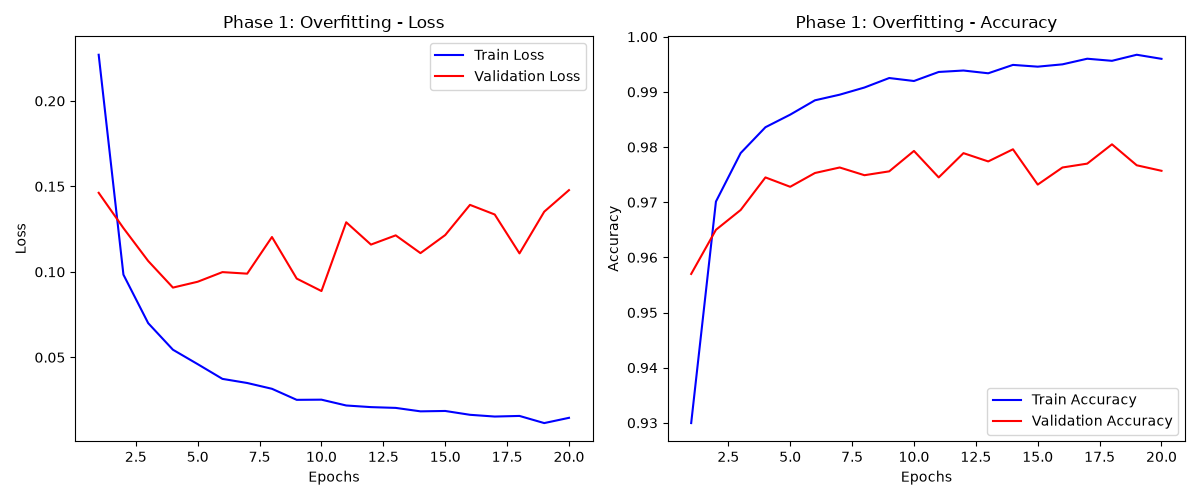
\includegraphics[width=0.9\textwidth]{phase_1_-_overfitting.png}
\caption{Training and Validation Curves Showing Overfitting}
\label{fig:overfit}
\end{figure}

%----------------------------------------

\subsection{Phase 2: Resolving Overfitting}

A new instance of the same neural network is trained using regularization techniques.

The following techniques are applied.

\begin{enumerate}

\item Data Augmentation

\item $L_2$ Regularization (Weight Decay)

\end{enumerate}

The optimizer uses

\[
Weight\ Decay = 1\times10^{-4}
\]

which penalizes large weights and prevents memorization.

\subsubsection*{Expected Result}

The model should

\begin{itemize}

\item Learn more generalized features

\item Reduce validation loss

\item Improve test accuracy

\item Reduce the gap between training and validation performance

\end{itemize}

\subsubsection*{Result}

The graph below illustrates the improvement after applying regularization.

\begin{figure}[H]
\centering
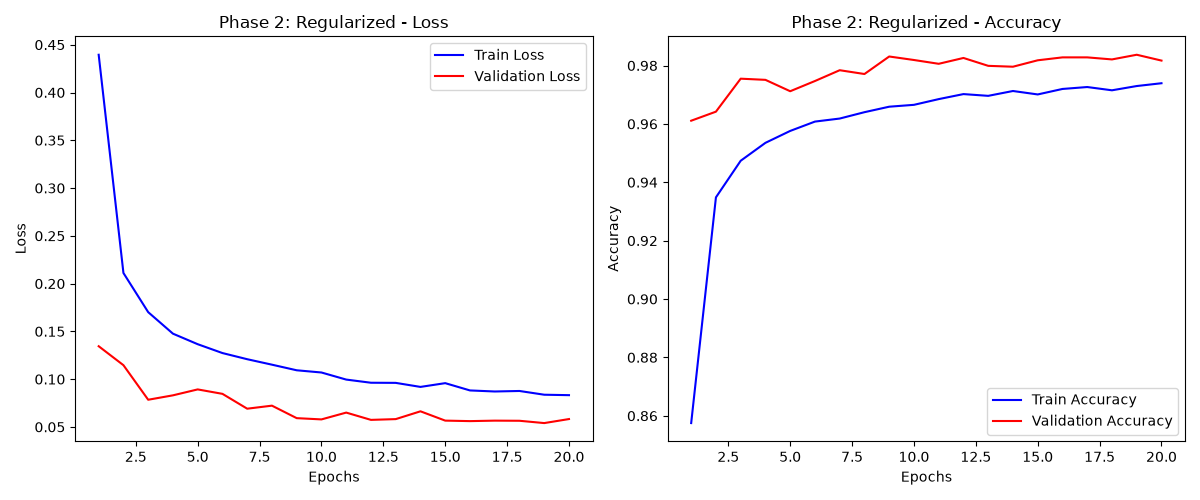
\includegraphics[width=0.9\textwidth]{phase_2_-_regularization.png}
\caption{Training and Validation Curves After Applying Data Augmentation and $L_2$ Regularization}
\label{fig:regularization}
\end{figure}

%----------------------------------------

\section{Discussion}

The comparison between both experiments clearly demonstrates the effect of overfitting.

Without regularization, the model memorizes the training data, resulting in poor performance on unseen data.

Applying Data Augmentation and $L_2$ Regularization forces the network to learn more meaningful features rather than memorizing individual samples.

Consequently, validation performance improves and the model generalizes better.

%----------------------------------------

\section{Conclusion}

This project successfully demonstrates both the occurrence of overfitting and the effectiveness of regularization techniques.

A high-capacity neural network was intentionally trained to memorize the MNIST dataset. The resulting gap between training and validation performance clearly illustrated overfitting.

By introducing Data Augmentation and $L_2$ Regularization, the model achieved significantly better generalization while maintaining high accuracy.

These techniques are widely used in modern deep learning systems because they improve robustness and reduce the likelihood of overfitting.

%----------------------------------------

\section{References}

\begin{enumerate}


\item MNIST Dataset

\url{http://yann.lecun.com/exdb/mnist/}

\end{enumerate}

\end{document}
